%%%%%%%%%%%%%%%%%%%%%%%%%%%%%%%%%%%%%%%%%%%%%%%%%%%%%%%%%%%%%%%%%%%%
%% I, the copyright holder of this work, release this work into the
%% public domain. This applies worldwide. In some countries this may
%% not be legally possible; if so: I grant anyone the right to use
%% this work for any purpose, without any conditions, unless such
%% conditions are required by law.
%%%%%%%%%%%%%%%%%%%%%%%%%%%%%%%%%%%%%%%%%%%%%%%%%%%%%%%%%%%%%%%%%%%%

% This theme was based on fibeamer theme 
% If you found any bugs please contact @karlosos
% This repository is hosted on github https://github.com/karlosos/zut-fibeamer/

\documentclass{beamer}
\usetheme[faculty=wi]{fibeamer}
\usepackage[utf8]{inputenc}
\usepackage[
  main=polish,
  polish
]{babel}

\title{Aula 12  - React}
\subtitle{Tópicos especiais em Sistemas}
\author{Prof. Juliana Costa Silva - juliana.silva@up.edu.br}

\usepackage{ragged2e}  % `\justifying` text
\usepackage{booktabs}  % Tables
\usepackage{tabularx}
\usepackage{tikz}      % Diagrams
\usetikzlibrary{calc, shapes, backgrounds}
\usepackage{amsmath, amssymb}
\usepackage{url}       % `\url`s
\usepackage{listings}  % Code listings
\frenchspacing
\begin{document}

%------------------------------------------------------------------------
  \frame[c]{\maketitle}
      \begin{frame}<beamer>
      \frametitle{O que veremos hoje}
      \tableofcontents
    \end{frame}
%------------------------------------------------------------------------
    \section{Revendo...}
    \begin{frame}{Revendo...}{O que já aprendemos?}
      
      \begin{itemize}
            \item Criamos um projeto node;
            \item Organizamos os controladores na pasta controllers;
            \item Configuramos ações de GET e POST para a rota \alert{movimento}.
            \item Enviamos dados em formato JSON
             \item Persistência de dados
             \item Manipulamos datas
             \item Fizemos as funções de busca,e update do nosso proejto;
       \end{itemize}
     \end{frame}
     %------------------------------------------------------------------------
\begin{frame}[label=proof]{O projeto da disciplina}
	\begin{itemize}
	\item Faremos um sistema de controle financeiro pessoal;
	\item Este sistema deve ter:
	\begin{itemize}
	\item Registro de gastos;
	\item Login de usuários;
	\item Registro de renda (salários - comissões - negócios);
	\item Registro de cartões de créditos;
	\item Registro de contas bancárias;
	\end{itemize}
	\end{itemize}
    \end{frame}
%------------------------------------------------------------------------
    \begin{frame}[label=lists]{Front End}
      \begin{columns}[onlytextwidth]
        \column{.5\textwidth}
          \begin{itemize}
            \item Faremos o front-end da nossa aplicação utilizando ReactJS 
            \item O ReactJS foi criado pelo Facebook para fazer renderização e layouts mais complexos dentro da web.
          \end{itemize}
        \column{.5\textwidth}
            
\includegraphics[width=60mm]{resources/aula12_1.png}\\
            \tiny{Logo ReactJS}
      \end{columns}
    \end{frame}

%------------------------------------------------------------------------
\section{NPX}
    \begin{frame}[label=lists]{NPX}
    \begin{exampleblock}{O que é NPX}
        	\begin{itemize}
	\item O npx é o executador de pacotes. 
	\item Ao invés de baixar o pacote e instalar globalmente na máquina, é possível declarar que não quero instalar, mas somente utiliza-lo no momento.
	\item Nesse caso, usamos o npx, que vai buscar o pacote no npm, vai baixar as dependências que precisa e executar.
	\item Depois exclui os itens baixasos e fica só com o resultado final;
	\item O que ficará será a pasta com o projeto inicial do react criado.
        	\end{itemize}
      \end{exampleblock}
    \end{frame}
%------------------------------------------------------------------------
    \begin{frame}[label=lists]{Criando o projeto ReactJS}

% \begin{columns}[onlytextwidth]
%        \column{.5\textwidth}
         Para realizar a criação do projeto ReactJS usaremos o comando \alert{npx create-react-app nomeDoApp}
         \begin{itemize}
         \item Antes crie uma pasta para o projetoe abra ela no VSCode;
         \item Após a criação do projeto navegue até a pasta criada com ocomando \alert{cd nomeDoApp};
         \item execute o comando para iniciar seu projeto \alert{npm start};
         \end{itemize}
%        \column{.5\textwidth}
	            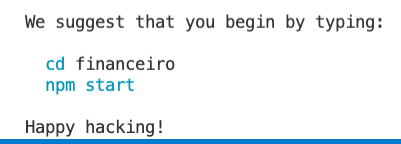
\includegraphics[width=80mm]{resources/aula12_2.png}\\
            \tiny{Resultado so comando! \textbf{Fonte:} O autor}
%      \end{columns}
    \end{frame}

%------------------------------------------------------------------------
    \begin{frame}[label=lists]{Auto reload}
          \begin{itemize}
            \item Para editar seu projeto não será necessário reiniciar o servidor;
            \item Ao salvar ele fará o auto reload.
          \end{itemize}
        
    \end{frame}
%------------------------------------------------------------------------
% \subsection{Referências}
%    \begin{frame}{Referências}%[allowframebreaks]
%\frametitle{Referências}
%\small
%\begin{center}
%\tiny
%\bibliographystyle{apalike}
%\bibliography{./ref_aula}
%\end{center}
%\end{frame}
  
\end{document}
